\documentclass[letterpaper,12pt]{book} %tipo de documento y tama~o de papel y letra

\usepackage{mystyle} %%Reemplazar por el contenido de 'mystyle.sty' en caso de no funcionar

\begin{document} %Inicio de documento
\begin{titlepage} %portada
\thispagestyle{empty} %borrar el formato de pagina linda
%\begin{flushleft} %alinear a la izq
\begin{center}

\includegraphics[scale=0.35]{logoUSM-DI.eps}
%\vfill
\end{center}
%\end{flushleft}

%\vspace{1cm} %espacio vertical , en realidad es un enter de 2 cm
\begin{center} %centrar
  {
    \begin{figure}[H]
      \centering
      \includegraphics[width=0.4\textwidth]{logo_Phyrex8.png}
      \label{fig:Phyrex}
    \end{figure}
    \Huge Plan de Proyecto\\
    \begin{figure}[H]
      \centering
      \includegraphics[width=0.2\textwidth]{VIPeR.png}
      \label{fig:Viper}
    \end{figure}
    \normalsize Santiago, 2013
  }
\end{center}

\vspace{1cm}

%\begin{figure}[H]
%  \centering
%  \begin{subfigure}[b]{0.4\textwidth}
%    \centering
%    \includegraphics[width=\textwidth]{logo_Phyrex8.png}
%    \label{fig:Phyrex}
%  \end{subfigure}
%  ~
%  \begin{subfigure}[b]{0.25\textwidth}
%    \centering
%    \includegraphics[width=\textwidth]{VIPeR.png}
%    \label{fig:Viper}
%  \end{subfigure}
%\end{figure}

\vfill
\begin{flushleft} %alinear izquierda
%  Pre-Empresa: \emph{Phyrex}
  Jefe de Proyecto: 
  \begin{table}[H]
    \centering
    \begin{tabular}{rll}
      Celeste Bertin     & \emph{Tel: +56 9 68410901} & \texttt{\small celeste.bertin@alumnos.usm.cl}  \\
    \end{tabular}          
  \end{table}              
  Integrantes:             
  \begin{table}[H]         
    \centering             
    \begin{tabular}{rll}   
      Rodrigo Fr\'{\i}as & \emph{Tel: +56 9 83988257} & \texttt{\small rodrigo.frias@alumnos.usm.cl}   \\
      Rocio Fernandez    & \emph{Tel: +56 9 62426549} & \texttt{\small rocio.fernandezu@alumnos.usm.cl}\\
      Juan Avalo         & \emph{Tel: +56 9 78072458} & \texttt{\small juan.avalo@alumnos.usm.cl}      \\
    \end{tabular}
  \end{table}
\end{flushleft}
\end{titlepage}

%    Patricio Carrasco &\texttt{\small <patricio.carrascod@alumnos.usm.cl>} &[+56 9 50626689]\\
 %Inclusion del titulo

\pagenumbering{Roman} %numero de paginas de indices en numeros romanos
\tableofcontents %indice de capitulos, secciones y subsecciones
\listoffigures   %indice de imagenes
\cleardoublepage
\listoftables    %indice de tablas
\cleardoublepage


%\chapter{Introducci\'on}

bla blablablablabalablablabalabalablba lab labla bal ablbdkjafnlajflsdjlgajsfl kamnslfkanslkganslkdfmsdkl f
g aodh ldgk dslg 

\pagenumbering{arabic} %numeracion en numeros arabicos
\setcounter{page}{1} %empezar enumerando la pagina 1
\part{Parte P\'ublica}            %% Parte Publica
\chapter{Material Formal}

\section{Introducci\'on} %Vision global del proyecto y de la experencia de llevarlo a cabo.

\section{Breve descripci\'on del Proyecto} %descripcion general del proyecto

\section{Resultado y futuro del Proyecto} %resultado final en que quedo su proyecto y posibles futuros, si los tiene
 %1. Material Formal
\section{T\'ecnicas y herramientas de desarrollo.}
Para el desarrollo de este proyecto, se ha decidido utilizar distintas metodolog\'ias y herramientas, muchas de las cuales son utilizadas dia a dia por miembros del equipo. 

\subsection{Modelo de desarrollo.}

Se ha decidido usar el modelo de desarrollo RUP (Rational Unified Process) para la implementaci\'on de este proyecto. RUP es un modelo que promueve el desarrollo iterativo y organiza la elaboraci\'on de software en 4 fases (inicio, elaboraci\'on, desarrollo y cierre) las cuales consisten de una o m\'as iteraciones ejecutables de este. 

\begin{figure}[H]
  \centering
  \includegraphics[scale=0.45]{Modelo.jpg}
%  \capture{}
  \label{fig:RUP}
\end{figure}

Este proyecto se separar\'a en cuatro secciones correspondientes a cada una de las entregas de ejecutables, las cuales se profundizar\'an en las cuatro iteraciones del ciclo de desarrollo. Las secciones son:

\begin{enumerate}
\item Funcionamiento b\'asico, dise\~no de robot
\item Implementaci\'on mascota virtual
\item Interacci\'on con robot
\item Interface, fluidez de interacci\'on entre mascota virtual y robot.
\end{enumerate}

De esta forma, se llevar\'an a cabo las distintas etapas de una manera iterativa, secuencial, modularizada e incremental.

Las especificaciones de los casos de uso y requerimientos se encuentran en el archivo Anexo.xlsx

\subsection{Herramientas y t\'ecnicas de soporte para el desarrollo.}

Para el desarrollo de Viper, el equipo Phyrex ha decidido utilizar las siguientes herramientas:

\begin{table}[H]
  \centering
  \begin{tabular}{|p{5cm}|p{9cm}|}\hline
    Herramientas & Detalle \\\hline\hline
    Sistema operativo android 2.1 o superior & Plataforma oficial de la aplicaci\'on\\
    Java & Lenguaje de programaci\'on usado para la aplicaci\'on de Android\\
    C & Lenguaje de programaci\'on usado para programar robot LEGO Mindstorms NXT\\
    UML & Lenguaje de modelado de base de datos\\
    Photoshop  & Herramienta de dise\~no gr\'afico\\
    LEGO Digital Designer & Herramienta de dise\~no y armado de estructuras de LEGO\\
    Google docs & Herramienta de edici\'on colaborativa de documentos\\
    Git & Herramienta de control de versiones\\
    Android SDK tools & Herramientas de desarrollo en Android\\
    Eclipse & Entorno de desarrollo para Android\\
    SQLite & Base de datos para la aplicaci\'on\\
    LEGO Mindstorms NXT & Robot programable de LEGO\\
    LEGO Mindstorms 2.0 & Ambiente de desarrollo para Mindstorms\\
    ROBOTC for LEGO Mindstorms & Ambiente de desarrollo para Mindstorms\\
    Skype & Herramienta de comunicaci\'on entre miembros del equipo\\
    Facebook & Herramienta para comunicaci\'on de noticias del proyecto\\
    \LaTeX & Edici\'on de documentos\\
    Microsoft Project & Herramienta de creaci\'on y manejo de carta gantt\\
    StarUML & Herramienta de modelado de casos de uso\\
    Trello & Herramienta de gesti\'on de proyectos\\\hline
  \end{tabular}
\end{table}

\subsection{Personal y capacitaci\'on del equipo de desarrollo.}

Para el desarrollo del proyecto, se necesita contar con un equipo que tenga conocimientos en Java para desarrollo en Android, SQLite, ROBOTC para LEGO Mindstorms, y Photoshop. 

El equipo de desarrollo para este proyecto es la pre-empresa Phyrex, una pre-empresa formada por cinco estudiantes de ingenier\'ia civil inform\'atica de la UTFSM, los cuales se presentan a continuaci\'on:

\begin{itemize}
\item {\bf Juan Avalo}: Experiencia en los lenguajes relevantes (Java, C). 
\item {\bf Celeste Bertin}: Experiencia previa en desarrollo en Android, aprendizaje r\'apido para resolver problemas nuevos. 
\item {\bf Patricio Carrasco}: Programador con experiencia en varios lenguajes.
\item {\bf Roc\'io Fern\'andez}: H\'abil dise\~nadora gr\'afica, experiencia previa en desarrollo en android, C y librer\'ia gr\'afica AndEngine, uso avanzado de LEGO. 
\item {\bf Rodrigo Fr\'ias}: Experiencia en maquetaci\'on de textos y programaci\'on en C.
\end{itemize}

El equipo esta en constante aprendizaje de Android para sacarle el mayor provecho a esta tecnolog\'ia. El equipo esta en capacitaci\'on de ROBOTC a trav\'es de tutoriales y documentaci\'on disponible en la web. 
 %2. Lecciones
\section{Gesti\'on de riesgos.}
 %3. Sugerencias
\section{Implementaci\'on (entrega y operaci\'on).}
 %4. Material Detallado de Apoyo
\part{Parte Privada}              %% Parte Privada
\section{Planificaci\'on de actividades.}
 %5. Aspectos Mejorables
\chapter{Comentarios Adicionales}

%si hay algun comentario o aporte que el equipo desea hacer dirigido solo a los profesores de los cursos y que no sera publicado en el futuro, debe hacerlo en esta seccion.
 %6. Comentarios Adicionales
%\appendix
\addappheadtotoc
\appendixpage

\chapter{Planificaci\'on de Actividades}
\label{appen:planificacion}

\newpage
\section[WBS]{Work Breakdown Structure}
\label{section:wbs}
El proyecto ser\'a realizado mediante la estructura \emph{RUP}. Cada actividad, a realizar en cada fase, tendr\'a un nivel de dificultad entre 1 y 5, siendo 5 la m\'as alta. Adem\'as, cada punto de dificultad quivaldr\'a a 4 Horas/Equipo (HE) y cada una de estas a 4 Horas/Hombre (HH).!

En las siguientes p\'aginas se muestra la estimaci\'on del esfuerzo estimado para el proyecto \emph{V.I.Pe.R.}:

\begin{table}[H]
  \centering
  \begin{tabular}{|l|m{5cm}|c|c|c|}\hline
    {\bf Fase} & {\bf Tarea} & {\bf Esfuerzo} & {\bf HE} & {\bf HH}\\\hline
    \multirow{4}{*}{Inicio} & Decisi\'on aplicaci\'on                & 3 & 12 & 48\\\cline{2-5}
           & Pruebas de robot                   & 3 & 12 & 48\\\cline{2-5}
           & Definici\'on software de desarrollo  & 2 & 12 & 48\\\cline{2-5}
           & Definici\'on nombre pre-empresa y producto & 2 & 8 & 32\\\hline
    \multirow{7}{*}{Elaboraci\'on} & Propuesta T\'ecnica           & 3 & 12 & 48\\\cline{2-5}
                & Toma de requisitos          & 5 & 20 & 80\\\cline{2-5}
                & Especificaci\'on casos de uso & 4 & 16 & 64\\\cline{2-5}
                & Identificaci\'on de riesgos   & 5 & 20 & 80\\\cline{2-5}
                & Mitigaci\'on de riesgos       & 5 & 20 & 80\\\cline{2-5}
                & P\'agina web                  & 3 & 12 & 48\\\cline{2-5}
                & Plan de proyecto            & 4 & 16 & 64\\\hline
    \multirow{5}{*}{Desarrollo} & Dise\~no de Interfaz                            & 5 & 20 & 100\\\cline{2-5}
               & Programaci\'on de Casos de Uso/Requerimientos   & -- & 75 & 300\\\cline{2-5}
               & Testing                                       & 3 & 12 & 60\\\cline{2-5}
               & Feedback                                      & 3 & 12 & 60\\\hline
                & {\bf Total}                 & -- & {\bf 279} & {\bf 1160}\\\hline
  \end{tabular}
  \label{tab:wbs}
  \caption[~Tabla WBS]{Divisi\'on de trabajo, seg\'un modelo utilizado, por esfuerzo.}
\end{table}


La que se resume, por fases, en la siguiente tabla:
\begin{table}[H]
\centering
\begin{tabular}{|l|c|c|c|}\hline
    {\bf Fase} & {\bf HE} & {\bf HH}\\\hline
    Inicio     & 44 & 176 \\\hline
    Elaboraci\'on & 116 & 464 \\\hline
    Desarrollo & 119 & 520 \\\hline
    {\bf Total} & {\bf 279} & {\bf 1160}\\\hline
\end{tabular}
\label{tab:fase}
\caption[~Distribuci\'on de horas para cada Fase]{Distribuci\'on de horas para cada Fase.}
\end{table}

\newpage
%CARTA GANTT
\section{Carta Gantt}
\label{appen:gantt}

%\includepdf[pagecommand={\section{Carta Gantt}},scale=0.7,pages=1,angle=-90,addtotoc={37,section,1,{Carta Gantt},appen:gantt}]{./pic/gantt.pdf}
%\includepdf[scale=0.7,pages=2-3,angle=-90,pagecommand={}]{./pic/gantt.pdf}

\begin{figure}[H]
\centering
\includegraphics[angle=-90,scale=0.7]{gantt1.eps}
\label{fig:gantt1}
\end{figure}

\begin{figure}[htbp!]
\centering
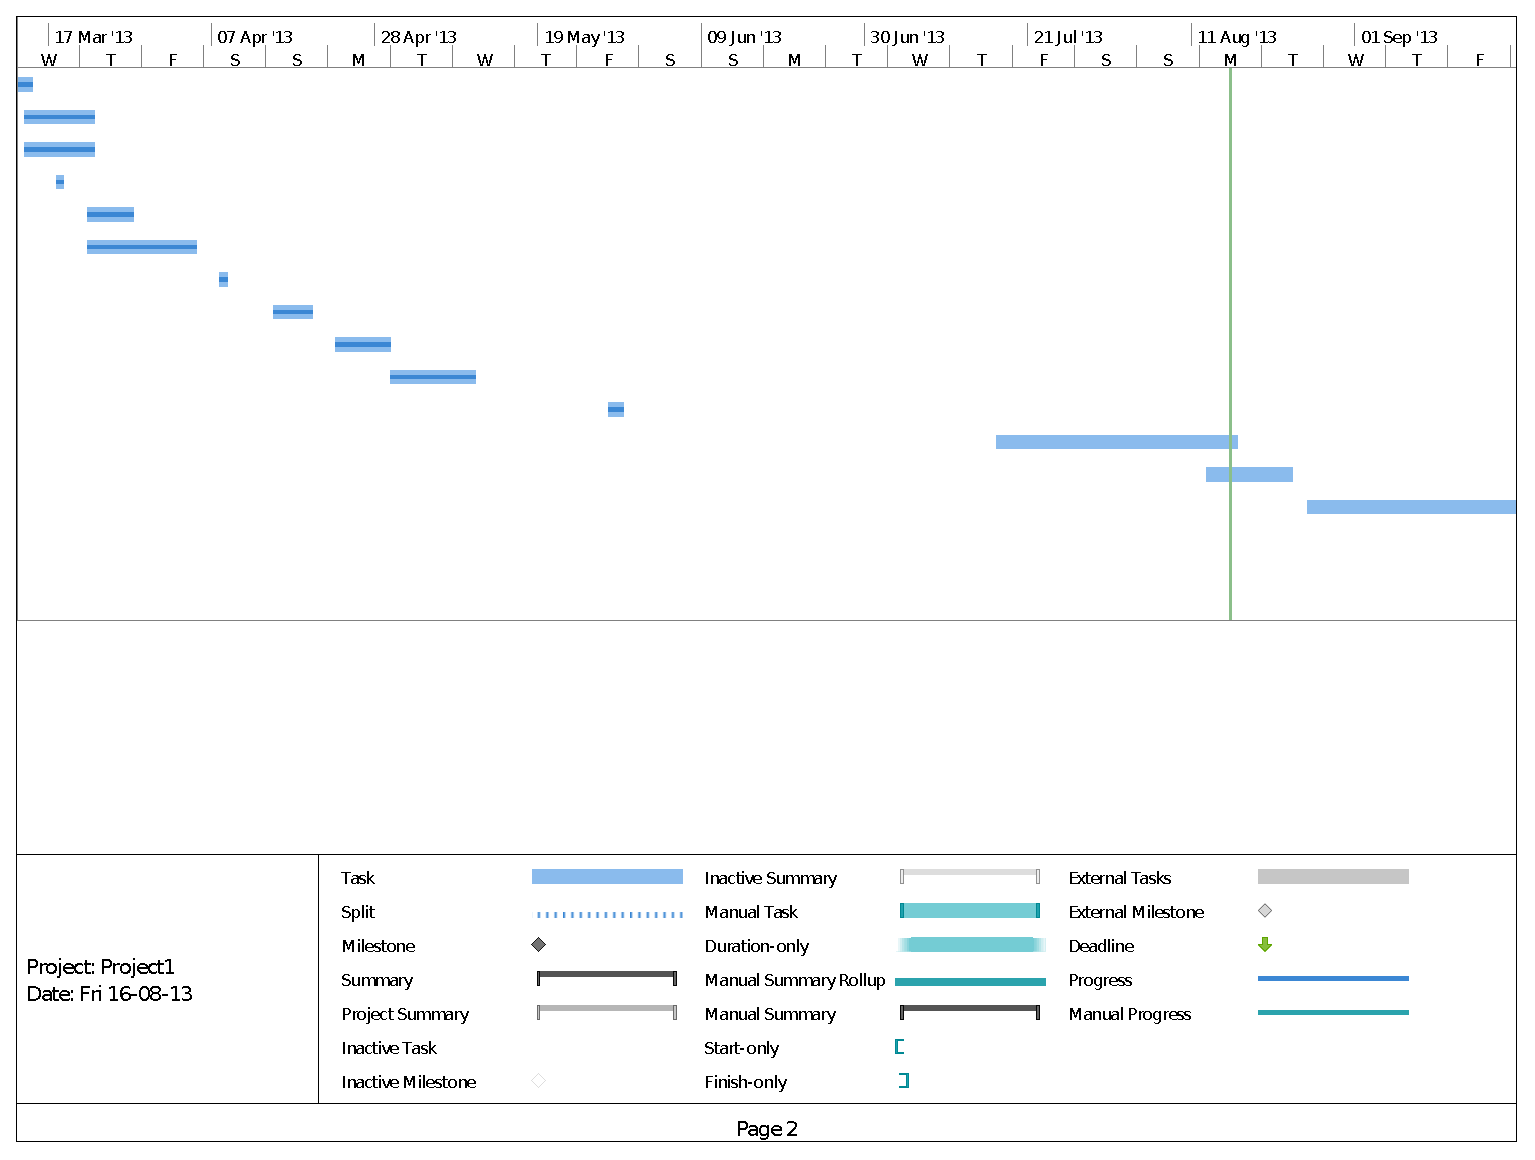
\includegraphics[angle=-90,scale=0.7]{gantt2.eps}
\label{fig:gantt2}
\end{figure}

\begin{figure}[htbp!]
\centering
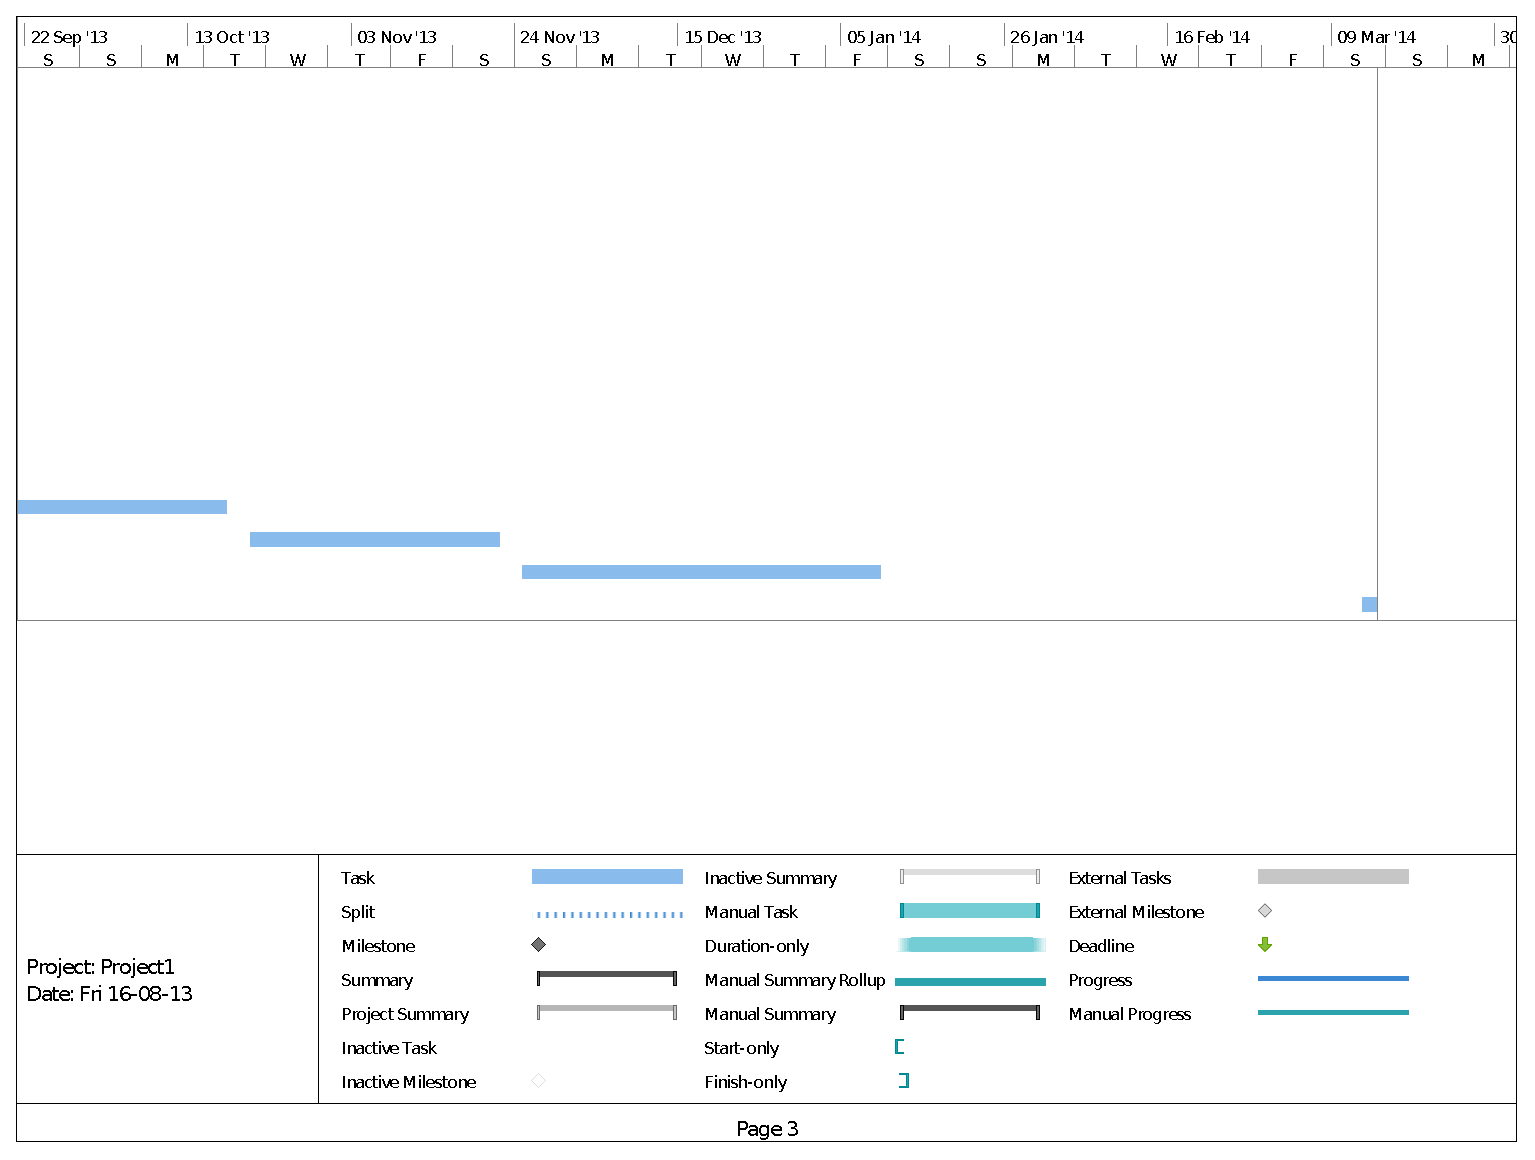
\includegraphics[angle=-90,scale=0.7]{gantt3.eps}
\label{fig:gantt3}
\end{figure}

%
%
%%Bibliografia
%\backmatter
%\addcontentsline{toc}{chapter}{Bibliograf\'ia}
%\bibliographystyle{acm}
%%%%%%%%%%%%%%%%%%%%%%%%%%%%%%%%%%%%%%%%%%%%%%%%%%%%%%%%%%%%%%%%%%%%%%%%%%%% 
% Bibliografía. 
%%%%%%%%%%%%%%%%%%%%%%%%%%%%%%%%%%%%%%%%%%%%%%%%%%%%%%%%%%%%%%%%%%%%%%%%%%% 
\begin{thebibliography}{99} 
  \bibitem{etiqueta-referencia1} Autor: \textit{T\'itulo}. Editorial, a\~no. 
  \bibitem{etiqueta-referencia2} Autor: \textit{T\'itulo}. Editorial, a\~no. 
\end{thebibliography}

\end{document}
